%%%%%%%%%%%%%%%%%%%%%%%%%%%%%%%%%%%%%%%%%%%%%%%%%%%%%%%%%%%
%%%%%%%%%%%%%%%%%%%%%%%%%%%%%%%%%%%%%%%%%%%%%%%%%%%%%%%%%%%
%%%%%%%%%%%%%%%%%%%%%%%%%%%%%%%%%%%%%%%%%%%%%%%%%%%%%%%%%%%

%% PREAMBLE! :-)


\documentclass[a4paper, 10pt]{article}

%%% packages - input should be path where your packages.tex file is saved.
%% packages

\usepackage{setspace}

%%%%%%%%%%%%%%%%%%%%%%%%%%%%%%%%%%%%%
\usepackage{sectsty}
\sectionfont{\sffamily\Large}
\subsectionfont{\sffamily}
%%%%%%%%%%%%%%%%%%%%%%%%%%%%%%%%%%%%%
\usepackage[titles]{tocloft}
%%%%%%%%%%%%%%%%%%%%%%%%%%%%%%%%%%%%%

%%% This is a package to use UTF8 CSV files as input and directly convert them to latex tables.
\usepackage{csvsimple}
%https://texblog.org/2012/05/30/generate-latex-tables-from-csv-files-excel/

%%%%%%%%%%%%%%%%%%%%%%%%%%%%%%%%%%%%%
%%%%%%%%%%%%%%%%%%%%%%%%%%%%%%%%%%%%%
%%%%%%%%%%%%%%%%%%%%%%%%%%%%%%%%%%%%%

\usepackage[version=4]{mhchem}
% package for using chemical equations and fonts 
% https://mirror.kumi.systems/ctan/macros/latex/contrib/mhchem/mhchem.pdf

%%%%%%%%%%%%%%%%%%%%%%%%%%%%%%%%%%%%%
%%%%%%%%%%%%%%%%%%%%%%%%%%%%%%%%%%%%%
%%%%%%%%%%%%%%%%%%%%%%%%%%%%%%%%%%%%%

\usepackage{xparse}
% high level user interface package, use with caution
% https://mirror.easyname.at/ctan/macros/latex/contrib/l3packages/xparse.pdf

%%%%%%%%%%%%%%%%%%%%%%%%%%%%%%%%%%%%%
%%%%%%%%%%%%%%%%%%%%%%%%%%%%%%%%%%%%%
%%%%%%%%%%%%%%%%%%%%%%%%%%%%%%%%%%%%%

\usepackage{makeidx}
\usepackage{pdfpages}
\usepackage{lastpage}

%%%%%%%%%%%%%%%%%%%%%%%%%%%%%%%%%%%%%
%%%%%%%%%%%%%%%%%%%%%%%%%%%%%%%%%%%%%
%%%%%%%%%%%%%%%%%%%%%%%%%%%%%%%%%%%%%

%%% Package to control inclusion and exclusion of specific entry in the table of contents.
%%% https://mirror.foobar.to/CTAN/macros/latex/contrib/tocbibind/tocbibind.pdf
\usepackage[nottoc,notlot,notlof]{tocbibind}

%%%%%%%%%%%%%%%%%%%%%%%%%%%%%%%%%%%%%
%%%%%%%%%%%%%%%%%%%%%%%%%%%%%%%%%%%%%
%%%%%%%%%%%%%%%%%%%%%%%%%%%%%%%%%%%%%

\usepackage{bigstrut}
% needed for crazy table commands, its cool trust me!
% https://anorien.csc.warwick.ac.uk/mirrors/CTAN/macros/latex/contrib/multirow/multirow.pdf

%%%%%%%%%%%%%%%%%%%%%%%%%%%%%%%%%%%%%
%%%%%%%%%%%%%%%%%%%%%%%%%%%%%%%%%%%%%
%%%%%%%%%%%%%%%%%%%%%%%%%%%%%%%%%%%%%

\usepackage{graphicx} 								
% Required for the inclusion of images
% https://de.overleaf.com/learn/latex/Inserting_Images

%%%%%%%%%%%%%%%%%%%%%%%%%%%%%%%%%%%%%
%%%%%%%%%%%%%%%%%%%%%%%%%%%%%%%%%%%%%
%%%%%%%%%%%%%%%%%%%%%%%%%%%%%%%%%%%%%

\usepackage{amsmath} 								
% Required for some math elements 
% https://www.namsu.de/Extra/pakete/amsmath/Amsmath.html

%%%%%%%%%%%%%%%%%%%%%%%%%%%%%%%%%%%%%
%%%%%%%%%%%%%%%%%%%%%%%%%%%%%%%%%%%%%
%%%%%%%%%%%%%%%%%%%%%%%%%%%%%%%%%%%%%

\usepackage{amssymb}
% required for some more crazy math elements, checks mal ab!
% http://milde.users.sourceforge.net/LUCR/Math/mathpackages/amssymb-symbols.pdf

%%%%%%%%%%%%%%%%%%%%%%%%%%%%%%%%%%%%%
%%%%%%%%%%%%%%%%%%%%%%%%%%%%%%%%%%%%%
%%%%%%%%%%%%%%%%%%%%%%%%%%%%%%%%%%%%%

%\usepackage{kbordermatrix} 	
% some special matrix-commands						
% http://www.hss.caltech.edu/~kcb/TeX/kbordermatrix.sty
%%%%%%%%%%%%%%%%%%%%%%%%%%%%%%%%%%%%%
%%%%%%%%%%%%%%%%%%%%%%%%%%%%%%%%%%%%%
%%%%%%%%%%%%%%%%%%%%%%%%%%%%%%%%%%%%%

\usepackage{multicol}								
% multicolumn-commands stuffs
% https://de.overleaf.com/learn/latex/Multiple_columns

%%%%%%%%%%%%%%%%%%%%%%%%%%%%%%%%%%%%%
%%%%%%%%%%%%%%%%%%%%%%%%%%%%%%%%%%%%%
%%%%%%%%%%%%%%%%%%%%%%%%%%%%%%%%%%%%%

\usepackage{color}
\definecolor{dkgreen}{rgb}{0,0.6,0}
\definecolor{gray}{rgb}{0.5,0.5,0.5}
\definecolor{mauve}{rgb}{0.58,0,0.82}
\definecolor{darkblue}{rgb}{0.0,0.0,0.6}
\definecolor{cyan}{rgb}{0.0,0.6,0.6}

%%%%%%%%%%%%%%%%%%%%%%%%%%%%%%%%%%%%%
%%%%%%%%%%%%%%%%%%%%%%%%%%%%%%%%%%%%%
%%%%%%%%%%%%%%%%%%%%%%%%%%%%%%%%%%%%%

% package to more precisely wrap your document around ur figure!
% https://de.overleaf.com/learn/latex/wrapping_text_around_figures
\usepackage{wrapfig}								

%%%%%%%%%%%%%%%%%%%%%%%%%%%%%%%%%%%%%
%%%%%%%%%%%%%%%%%%%%%%%%%%%%%%%%%%%%%
%%%%%%%%%%%%%%%%%%%%%%%%%%%%%%%%%%%%%

% the package for bold math symbol commands!
% https://anorien.csc.warwick.ac.uk/mirrors/CTAN/macros/latex/required/tools/bm.pdf
\usepackage{bm}

%%%%%%%%%%%%%%%%%%%%%%%%%%%%%%%%%%%%%
%%%%%%%%%%%%%%%%%%%%%%%%%%%%%%%%%%%%%
%%%%%%%%%%%%%%%%%%%%%%%%%%%%%%%%%%%%%

% subcaption package dependant on caption package (self-explanatory)
% https://www.namsu.de/Extra/pakete/Subcaption.html

\usepackage{caption}
\usepackage{subcaption}

%%%%%%%%%%%%%%%%%%%%%%%%%%%%%%%%%%%%%
%%%%%%%%%%%%%%%%%%%%%%%%%%%%%%%%%%%%%
%%%%%%%%%%%%%%%%%%%%%%%%%%%%%%%%%%%%%

%package for appendix control
% https://mirror.easyname.at/ctan/macros/latex/contrib/appendix/appendix.pdf
\usepackage[toc,page]{appendix}

%%%%%%%%%%%%%%%%%%%%%%%%%%%%%%%%%%%%%
%%%%%%%%%%%%%%%%%%%%%%%%%%%%%%%%%%%%%
%%%%%%%%%%%%%%%%%%%%%%%%%%%%%%%%%%%%%

% This is the listings package to make code appear like actual code!
% https://mirror.foobar.to/CTAN/macros/latex/contrib/listings/listings.pdf
\usepackage{listings}{
 \lstset{frame=tb,
  basicstyle=\fontsize{9}{11}\selectfont\sffamily,
  frame=single,	 
  language=Python,
  breaklines=true,
  showstringspaces=false,
  columns=flexible,
  numbers=left,
  commentstyle=\color{dkgreen},
  stringstyle=\color{mauve},
  tabsize=2
}

%%%%%%%%%%%%%%%%%%%%%%%%%%%%%%%%%%%%%
%%%%%%%%%%%%%%%%%%%%%%%%%%%%%%%%%%%%%
%%%%%%%%%%%%%%%%%%%%%%%%%%%%%%%%%%%%%

% this package for more elaborate appendix commands!
% http://mirror.ox.ac.uk/sites/ctan.org/macros/latex/contrib/appendix/appendix.pdf
\usepackage[toc,page]{appendix}
%\renewcommand{\appendixpagename}{\appendixname}
%\renewcommand{\appendixtocname}{\appendixname}

%%%%%%%%%%%%%%%%%%%%%%%%%%%%%%%%%%%%%
%%%%%%%%%%%%%%%%%%%%%%%%%%%%%%%%%%%%%
%%%%%%%%%%%%%%%%%%%%%%%%%%%%%%%%%%%%%

% this is the hyperlink references package! To make stuff in your text clickable and send you to the right page, URL's, E-mails etc..
% http://mirror.ox.ac.uk/sites/ctan.org/macros/latex/contrib/hyperref/doc/manual.pdf
\usepackage[
    bookmarks,
    bookmarksopen=true,
    colorlinks=true,			% diese Farbdefinitionen zeichnen Links im PDF farblich aus
    linkcolor=black, 			% einfache interne Verknüpfungen
    anchorcolor=black,			% Ankertext
    citecolor=black, 			% Verweise auf Literaturverzeichniseinträge im Text
    filecolor=magenta, 			% Verknüpfungen, die lokale Dateien öffnen
    menucolor=red, 				% Acrobat-Menüpunkte
    urlcolor=blue,				% URL color of course :P
    plainpages=false,		 	% zur korrekten Erstellung der Bookmarks
    pdfpagelabels, 				% zur korrekten Erstellung der Bookmarks
    hypertexnames=true, 		% zur korrekten Erstellung der Bookmarks
    %linktocpage 				% Seitenzahlen anstatt Text im Inhaltsverzeichnis verlinken
]{hyperref}

\usepackage{tcolorbox}
%Fancy boxes around text!
%%%%%%%%%%%%%%%%%%%%%%%%%%%%%%%%%%%%%

\usepackage{amsthm}
\usepackage{algorithm}
\usepackage{algpseudocode}
\usepackage{tikz}

%%% Settings!
%% settings
%change relevant macros like title, names etc.

\newcommand{\firstauthorfirstname}{Camilo }
\newcommand{\firstauthorlastname}{Tello Fachin }

\newcommand{\secondauthorfirstname}{Second }
\newcommand{\secondauthorlastname}{Author }

\newcommand{\doctitle}{Exercise 5}

\makeindex
%%%%%%%%%%%%%%%%%%%%%%%%%%%%%%%%%%%%%%%%%%%%%%%%%%%%%%%%%%%%%%%%%%%%%%%%%
%%%%%%%%%%%%%%%%%%%%%%%%%%%%%%%%%%%%%%%%%%%%%%%%%%%%%%%%%%%%%%%%%%%%%%%%%
%%%%%%%%%%%%%%%%%%%%%%%%%%%%%%%%%%%%%%%%%%%%%%%%%%%%%%%%%%%%%%%%%%%%%%%%%

% set the margins of the document, single first input generates evenly spaced margins of that value
\usepackage[margin=2.5cm]{geometry}

%%%%%%%%%%%%%%%%%%%%%%%%%%%%%%%%%%%%%%%%%%%%%%%%%%%%%%%%%%%%%%%%%%%%%%%%%
%%%%%%%%%%%%%%%%%%%%%%%%%%%%%%%%%%%%%%%%%%%%%%%%%%%%%%%%%%%%%%%%%%%%%%%%%
%%%%%%%%%%%%%%%%%%%%%%%%%%%%%%%%%%%%%%%%%%%%%%%%%%%%%%%%%%%%%%%%%%%%%%%%%

\usepackage[utf8]{inputenc}
% u need this one to compile ä ö ü while babel-package is disabled!(english document)!!
% https://www.namsu.de/Extra/pakete/Inputenc.html

%\usepackage[ngerman]{babel}
% uncomment this package to have all the generated text lik TOC and TOC-APP in german
% IF U UNCOMMENT THIS, PUT THE UTF8 INPUTENC PACKAGE IN COMMENT
% https://www.namsu.de/Extra/pakete/German.html

%%%%%%%%%%%%%%%%%%%%%%%%%%%%%%%%%%%%%%%%%%%%%%%%%%%%%%%%%%%%%%%%%%%%%%%%%
%%%%%%%%%%%%%%%%%%%%%%%%%%%%%%%%%%%%%%%%%%%%%%%%%%%%%%%%%%%%%%%%%%%%%%%%%
%%%%%%%%%%%%%%%%%%%%%%%%%%%%%%%%%%%%%%%%%%%%%%%%%%%%%%%%%%%%%%%%%%%%%%%%%


% header and footer settings
% to look up stuff on it go visit this one:
% https://en.wikibooks.org/wiki/LaTeX/Customizing_Page_Headers_and_Footers

\usepackage{fancyhdr}
\setlength{\headheight}{22.25pt}

\renewcommand{\headrulewidth}{0.5pt}
\renewcommand{\footrulewidth}{0.5pt}

\pagestyle{fancy}


% header inputs
\lhead[even output]{CSMCA}
\chead[even output]{Exercise 5}
\rhead[even output]{
\includegraphics[width=2.5cm]{figures/uni_header}}


%footer inputs
\lfoot[even output]{CSE - WS22}
\cfoot[even output]{Page  \thepage}
\rfoot[even output]{\today}

%%%%%%%%%%%%%%%%%%%%%%%%%%%%%%%%%%%%%%%%%%%%%%%%%%%%%%%%%%%%%%%%%%%%%%%%%
%%%%%%%%%%%%%%%%%%%%%%%%%%%%%%%%%%%%%%%%%%%%%%%%%%%%%%%%%%%%%%%%%%%%%%%%%
%%%%%%%%%%%%%%%%%%%%%%%%%%%%%%%%%%%%%%%%%%%%%%%%%%%%%%%%%%%%%%%%%%%%%%%%%


%settings for PDF metadata, available if rightclick on pdf in adobe and chose properties!

\hypersetup{pdfinfo={
Title={\doctitle},
Subject={Computational Science on Many Core Architectures},
Author={Camilo Tello Fachin},
Keywords={C++, }{Cuda, }{Technical University Vienna, }{Winter Semester 22, }
{MSc Computational Science and Engineering}
}}

%%%%%%%%%%%%%%%%%%%%%%%%%%%%%%%%%%%%%%%%%%%%%%%%%%%%%%%%%%%%%%%%%%%%%%%%%
%%%%%%%%%%%%%%%%%%%%%%%%%%%%%%%%%%%%%%%%%%%%%%%%%%%%%%%%%%%%%%%%%%%%%%%%%
%%%%%%%%%%%%%%%%%%%%%%%%%%%%%%%%%%%%%%%%%%%%%%%%%%%%%%%%%%%%%%%%%%%%%%%%%

%% This is the bibliography package,
\usepackage[
backend=bibtex,
style=ieee,
sorting=ynt,
backref=false,
hyperref=true
]{biblatex}

%%%%%%%%%%%%%%%%%%%%%%%%%%%%%%%%%%%%%%%%%%%%%%%%%%%%%%%%%%%%%%%%%%%%%%%%%
%%%%%%%%%%%%%%%%%%%%%%%%%%%%%%%%%%%%%%%%%%%%%%%%%%%%%%%%%%%%%%%%%%%%%%%%%
%%%%%%%%%%%%%%%%%%%%%%%%%%%%%%%%%%%%%%%%%%%%%%%%%%%%%%%%%%%%%%%%%%%%%%%%%

%%% This is an important setting which lets u control the spacing between lines! Just comment/uncomment the desired ones!


%\singlespacing

\onehalfspacing

%\doublespacing

%%%%%%%%%%%%%%%%%%%%%%%%%%%%%%%%%%%%%%%%%%%%%%%%%%%%%%%%%%%%%%%%%%%%%%%%%

%%% custom commands

\newcommand{\var}[1]{\texttt{#1}}
\newcommand{\fun}[1]{\texttt{#1}}
\newcommand{\obj}[1]{\texttt{#1}}

\newtheorem*{theorem*}{Theorem}
\newtheorem*{proof*}{Proof}

%%% macros - where u define ur macros and newcommands!
% useful macros!


% insert a blank page which is still counted
\newcommand{\blankpage}{
\newpage
\thispagestyle{empty}
\mbox{}
\newpage
}

%%% the bibliohraphy! the settings to the bibliography are changed in the packages.tex file, where the bibtex package is loaded!
\addbibresource{content/04_bibliography.bib}

\begin{document}


%%%%%%%%%%%%%%%%%%%%%%%%%%%%%%%%%%%%%%%%%%%%%%%%%%%%%%%%%%%
%%%%%%%%%%%%%%%%%%%%%%%%%%%%%%%%%%%%%%%%%%%%%%%%%%%%%%%%%%%%
%%%%%%%%%%%%%%%%%%%%%%%%%%%%%%%%%%%%%%%%%%%%%%%%%%%%%%%%%%%
          

\begin{titlepage}

\newcommand{\HRule}{\rule{\linewidth}{0.5mm}} % Defines a new command for the horizontal lines, change thickness here

\center % Center everything on the page
 
%----------------------------------------------------------------------------------------
%	HEADING SECTIONS
%----------------------------------------------------------------------------------------

\textsc{\LARGE Vienna University of Technology}\\[1.5cm] % Name of your university/college
\textsc{\Large 360.252 Computational Science on Many Core Architectures}\\[0.5cm] % Major heading such as course name
\textsc{\large Institute for Microelectronics}\\[0.5cm] % Minor heading such as course title

%----------------------------------------------------------------------------------------
%	TITLE SECTION
%----------------------------------------------------------------------------------------

\HRule \\[0.5cm]
{ \huge \bfseries \doctitle}\\[1mm] % Title of your document
\HRule \\[0.5cm]
 
%----------------------------------------------------------------------------------------
%	AUTHOR SECTION
%----------------------------------------------------------------------------------------

\begin{minipage}{0.4\textwidth}
\begin{flushleft} \large
\emph{Authors:}\\
Camilo \textsc{Tello Fachin}\\
12127084 \\

\end{flushleft}
\end{minipage}
~
\begin{minipage}{0.4\textwidth}
\begin{flushright} \large
\emph{Supervisor:} \\
Dipl.-Ing. Dr.techn. Karl \textsc{Rupp} \\ % Supervisor's Name
\end{flushright}
\end{minipage}\\[1.5cm]

% If you don't want a supervisor, uncomment the two lines below and remove the section above
%\Large \emph{Author:}\\
%John \textsc{Smith}\\[3cm] % Your name

%----------------------------------------------------------------------------------------
%	DATE SECTION
%----------------------------------------------------------------------------------------

{\large \today}\\[1.5cm] % Date, change the \today to a set date if you want to be precise

%----------------------------------------------------------------------------------------
%	LOGO SECTION
%----------------------------------------------------------------------------------------
\vfill


\includegraphics[width=0.75\textwidth]{figures/uni_titlepage}\\[5cm] % Include a department/university logo
 
%----------------------------------------------------------------------------------------

\vfill % Fill the rest of the page with whitespace
\pagenumbering{alph}

\end{titlepage} 

%\blankpage

% this is to remove the first paragraph sentence indentation! if you want indentation, set the second input to the desired indendation value.
\setlength{\parindent}{0pt}

% this file is loaded, to include PDF's such as declaration of intent for theses, abstracts and summaries in other languages.
\pagenumbering{roman}

\section*{Abstract}
Dear Professor Rupp. Tried handing in some stuff before midnight, the plot for 1.a!
It is not finished, but I handed something in before 23:59, I hope you appreciate the loophole identified by me enough to grant me the point!
See you soon and have a nice evening. Camilo Tello Fachin



%%% If your TOC is too large for one page, you can distribute it over 2 pages and comment this /blankpage command below! To better control the distribution of the content of the table of content, use the geometry settings and adjust the top and bottom margin for the table of content in the next part of this code.

%\blankpage



%%% Here u define the TOC, a newgeometry command is used to let you design your own TOC margins. just comment out the \newgeometry and the \restoregeometry
%%% command to force the same margins as the rest of the document to the TOC

\pagebreak
\thispagestyle{empty}
\newgeometry{top=2.25cm, bottom=2.25cm}
{\sffamily\tableofcontents}
\thispagestyle{empty}
\restoregeometry
\pagebreak

\pagenumbering{arabic}


%%%%%%%%%%%%%%%%%%%%%%%%%%%%%%%%%%%%%%%%%%%%%%%%%%%%%%%%%%%
%%%%%%%%%%%%%%%%%%%%%%%%%%%%%%%%%%%%%%%%%%%%%%%%%%%%%%%%%%%
%%%%%%%%%%%%%%%%%%%%%%%%%%%%%%%%%%%%%%%%%%%%%%%%%%%%%%%%%%%
%%%%%%%%%%%%%%%%%%%%%%%%%%%%%%%%%%%%%%%%%%%%%%%%%%%%%%%%%



%%% This is a first surrogate chapter to intuitively show you how and where to include new chapters!
%\section*{To Do's}

- What's still to you do make your supervisor/prof happy?
\pagebreak





%\pagebreak

\section{Chapter 1}

\begin{figure}[h]
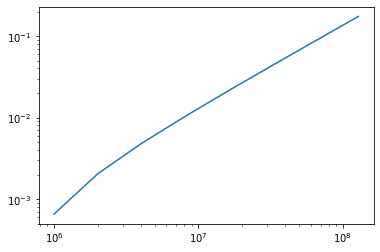
\includegraphics[width=1\textwidth]{figures/output.png}
\end{figure}
%\pagebreak

%\section{HIP (Points 3/3)}
Successfully Implemented the classical CG Algorithm in HIP. Whereby "implmenting" I mean replacing \fun{CUDA} commands to \fun{HIP} commands.
A bit trickier where the Kernel calls, But eventually made it run and it still converges and yields corrects results (Relative residual error smaller than 1e-6).

\begin{figure}[h]
    \begin{center}
        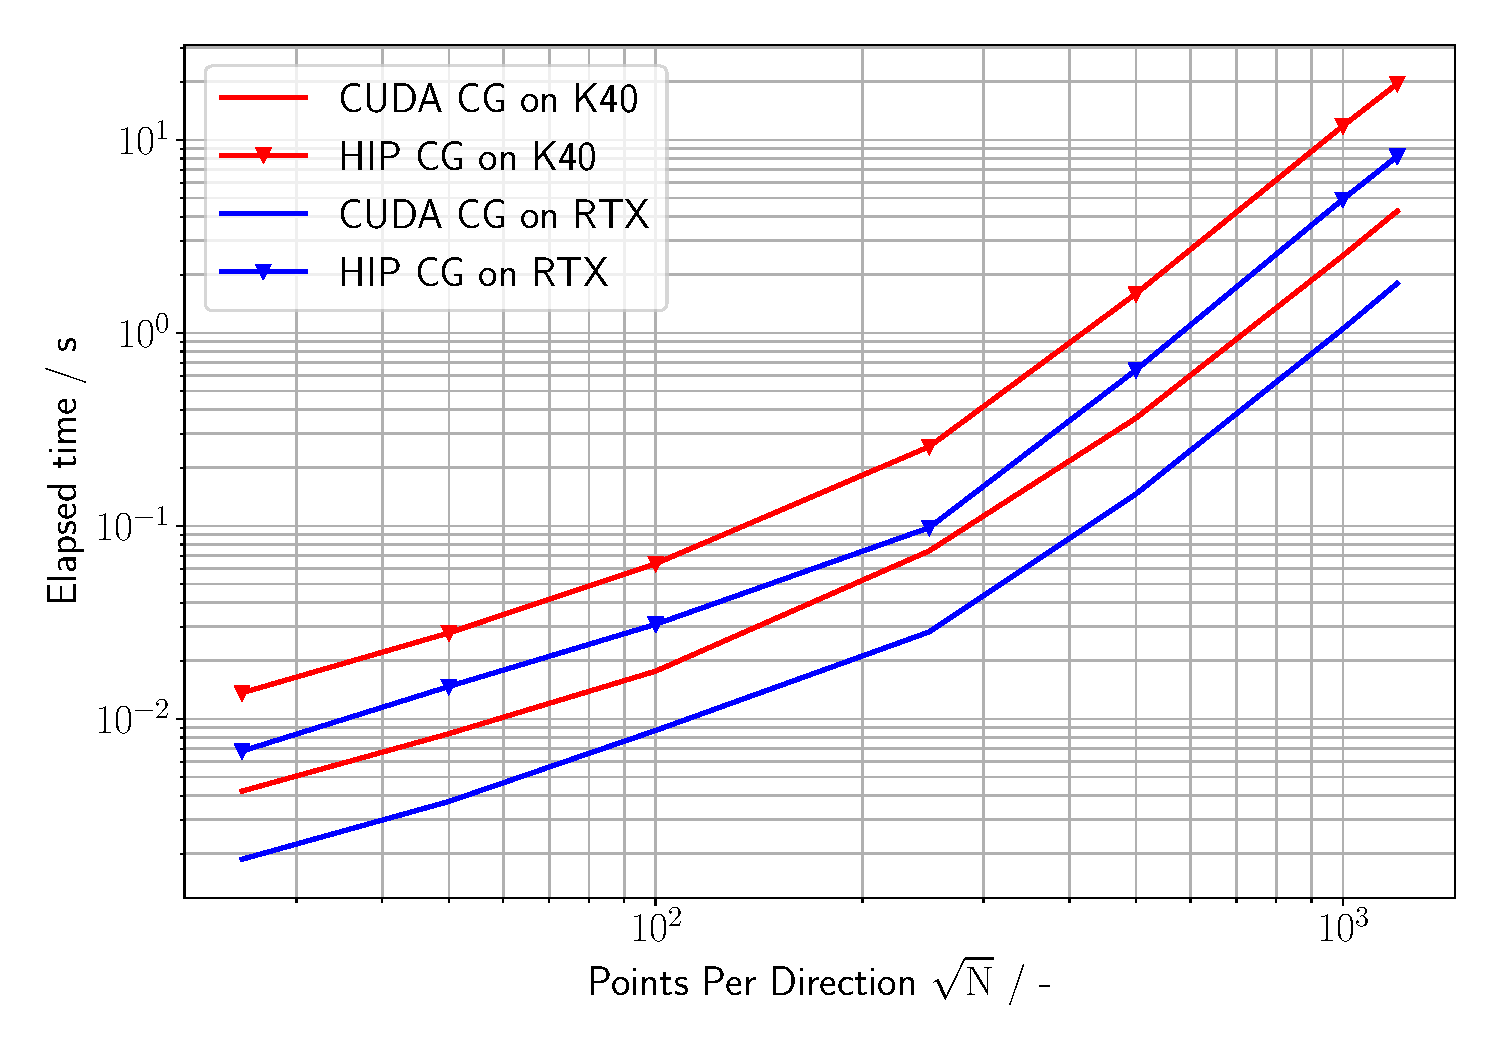
\includegraphics[width = \linewidth]{figures/task_9_2_plot.pdf}
        \caption{Comparison Conjugate Gradient Algorithm with \fun{CUDA} and \fun{HIP}}
        \end{center}
\end{figure}

The HIP Implementation is slower for both GPU's!

\section{BONUS: Relaxed Christmas Break (0/1 Point)}
I had a very relaxed christmas break, therefore You could grant me the Bonus point!
Jokes aside, I hope You had a very relaxed Christmas break! :-) Kind regards.

%\pagebreak

%\section{Chapter 3}
\subsection{Proof and Theorem Environment Example}

As explained in the introduction, the existence of the shape derivative needs to be shown.
The perturbations of the shape $\Omega$ are described by the transformation: $\Omega_t := (Id + tX )(\Omega)$ 
For small perturbations and $t > 0$, the shape derivative is \cite{fully_semi_paper_sturm}

\begin{equation}\label{shape_derrivative_t_limit}
	DJ(\Omega)(X) := \left(\frac{\partial}{\partial t}J(\Omega_t)\right)\bigg\rvert_{t=0} = \lim_{t \to 0} \frac{J(\Omega_t)-J(\Omega)}{t}.
\end{equation}
This notion of the shape derivative is used in this chapter in the context of differentiability. The functional $J(\Omega)$ that returns a scalar quantity 
represetative of the energy dissipation is shown here where : is the Frobenius product and $\mathrm{D} \mathbf{u}$ is the Jacobi matrix of $\mathbf{u}$.
\begin{align}\label{energy_dissipation_equation}
	J(\Omega) = \frac{1}{2} \int_{\Omega} \mathrm{D} \mathbf{u} : \mathrm{D} \mathbf{u} \, \mathrm{dx}.
\end{align}
Sturm et. al. \cite{nearly_conformal_paper} proposed the following shape derivative. \\
\begin{theorem*}
The Shape Derivative of $J$ at $\Omega$ in direction $ X \in [C^{0,1}(\bar{\Omega})]^2 $ is given by:
\begin{align}\label{shape_derivative_S1}
	\mathrm{d}J(\Omega)(X) &= \int_{\Omega} \mathrm{S}_1 : \mathrm{D}X \, \mathrm{dx}, \\
	\mathrm{S}_1 &= \left( \frac{1}{2}\mathrm{D} \mathbf{u} : \mathrm{D} \mathbf{u} - p \, \mathrm{div}(\mathbf{u}) \right)
	\mathrm{I}_2 + \mathrm{D} \mathbf{u}^{\top}p - \mathrm{D} \mathbf{u}^{\top} \mathrm{D} \mathbf{u}.
\end{align}
where $(\mathbf{u},p)$ solve (\ref*{weak_stokes_PDE_product})
\end{theorem*}
\begin{proof*}
let $X \in [C^{0,1}(\bar{\Omega})]^2$ with $X \rvert_{\Gamma_{\infty}} = 0$ be a given vectorfield. \\
Set $\mathrm{T}_t(.) := \mathrm{id} + tX $ , with $t \in \mathbb{R}$ and $\Omega_t := \mathrm{T}_t(\Omega)$, where 
$(\mathbf{u}_t, p_t)$ solve (\ref{weak_stokes_PDE_product}) and $\Omega$ is replaced by $\Omega_t$ s.t. \\
$p_t \in \mathrm{L}^2(\Omega_t), \int_{\Omega_t} p_t \, \mathrm{dx} = 0 $ and $\mathrm{u}_t \in [H^1(\Omega_t)]^2$. Then there holds 
\begin{align}
	\int_{\Omega_t} \mathrm{D} \mathbf{u}_t : \mathrm{D} \mathbf{\mathbf{v}} + \mathrm{div}(\mathbf{v}) \, p_t + \mathrm{div}(\mathbf{u}_t) \, q \, dx = \, 0 \quad \forall (v,q)
    \in  [H^1_0(\Omega_t)]^d \times L^2(\Omega_t).
\end{align}
Introduction of change of variables shows that $(\mathbf{u}^t, p^t) := (\mathbf{u}_t \circ \mathrm{T}_t, p_t \circ \mathrm{T}_t)$ satisfy
\begin{equation}
\begin{aligned}\label{trafo_weak_stokes}
	&\int_\Omega \mathrm{det}(\mathrm{DT}_t)
	\left( \mathrm{DT}_t^{-1} \mathrm{D}\mathbf{u}^t:\mathrm{DT}_t^{-1} \mathrm{D}\mathbf{v} -p\, \mathrm{tr}(\mathrm{D}\mathbf{v}\mathrm{DT}_t^{-1})  +
	q \, \mathrm{tr}(\mathrm{D}\mathbf{u}\mathrm{DT}_t^{-1}) \right) \mathrm{dx}, \\
	& \quad \quad \quad \quad \quad \quad \quad \quad \quad \ \forall (v,q) \in [H^1(\Omega)]^2 \times L^2(\Omega),
\end{aligned}
\end{equation}
Used in equation (\ref{trafo_weak_stokes})
\begin{align*}
	\mathrm{D}\mathbf{v}\circ\mathrm{T}_t &= \mathrm{D}(\mathbf{v}\circ\mathrm{T}_t), \\
	\mathrm{div}(\mathbf{v}) &= \mathrm{tr} \left( \mathrm{D}(\mathbf{v} \circ \mathrm{T}_t)(\mathrm{DT}_t^{-1}) \right).
\end{align*}

\vfill

\pagebreak

The functional $J(\Omega,\mathbf{u})$ is now reduced to the functional $J(\Omega)$, since the change of the quantities $(\mathbf{u},p)$
is taken into account by the transformation theorem. The minimum of (\ref{energy_dissipation_equation})
satisfies the saddlepoint problem (\ref{trafo_weak_stokes}). It can be obtained with the Lagrange Multiplier method, 
see Faustmann \cite{lecture_notes_faustmann_numPDE}. The corresponding Lagrangian which can be used to minimize (\ref{energy_dissipation_equation})
is
\begin{equation}\label{parametrized_lagrangian}
 \begin{aligned}
	\mathcal{L}(t,\mathbf{v}, q) = \frac{1}{2}& \int_{\Omega} \mathrm{det}(\mathrm{DT}_t) \mathrm{D} \mathbf{v}(\mathrm{DT}_t)^{-1} :
	\mathrm{D} \mathbf{v}(\mathrm{DT}_t)^{-1} \, \mathrm{dx}, \\
	&- \int_{\Omega}\mathrm{det}(\mathrm{DT}_t)q \, \mathrm{tr} \left( \mathrm{D}\mathbf{v}(\mathrm{DT}_t)^{-1} \right).
\end{aligned}
\end{equation}
To find the shape derivative, one can now derive this parametrized Lagrangian, for details on the derivation of parametrized Lagrangians, 
see K. Ito et. al. \cite{lagrangian_derivative}. With the derivative of the Lagrangian obtained, it holds true that
\begin{align}
	\mathrm{d}J(\Omega)(X) =\ \frac{\mathrm{d}}{\mathrm{d}t} \mathcal{L}(t, \mathbf{u}^t, 0)\big\rvert_{t=0}  =
	\frac{\partial}{\partial t}\mathcal{L}(0,\mathbf{u},p) = \int_{\Omega} \mathrm{S}_1 : \mathrm{D}X \, \mathrm{dx}.
\end{align}
\qed
\end{proof*}

%\pagebreak

%\section{Chapter 4}



%\pagebreak

%\section{Chapter 5}



%\pagebreak

%\section{Chapter 6}

%\pagebreak

%\section{Chapter 7}

%\pagebreak

%\section{Results and Conclusion}


%\pagebreak
%%%%%%%%%%%%%%%%%%%%%%%%%%%%%%%%%%%%%%%%%%%%%%%%%%%%%%%%%%%
%%%%%%%%%%%%%%%%%%%%%%%%%%%%%%%%%%%%%%%%%%%%%%%%%%%%%%%%%%%
%%%%%%%%%%%%%%%%%%%%%%%%%%%%%%%%%%%%%%%%%%%%%%%%%%%%%%%%%%%
%%%%%%%%%%%%%%%%%%%%%%%%%%%%%%%%%%%%%%%%%%%%%%%%%%%%%%%%%%%


%% During the document writing process, this single .tex file is used to let dasdyou write down a little to do list, just comment it out when the paper is done!

%%%%%%%%%%%%%%%%%%%%%%%%%%%%%%%%%%%%%%%%%%%%%%%%%%%%%%%%%%%
%%%%%%%%%%%%%%%%%%%%%%%%%%%%%%%%%%%%%%%%%%%%%%%%%%%%%%%%%%%
%%%%%%%%%%%%%%%%%%%%%%%%%%%%%%%%%%%%%%%%%%%%%%%%%%%%%%%%%%%
%%%%%%%%%%%%%%%%%%%%%%%%%%%%%%%%%%%%%%%%%%%%%%%%%%%%%%%%%

%%% Bibliography printing at this point! 
\printbibliography

%%% This is a hardcoded string to enforce it in the table of contents, if you want your "references" string in the TOC to be named differently, such as bibliography or so on, just change the third input to this command below to your desired references naming that should appear in the TOC
\addcontentsline{toc}{section}{References}


\pagebreak

%%%%%%%%%%%%%%%%%%%%%%%%%%%%%%%%%%%%%%%%%%%%%%%%%%%%%%%%%%%
%%%%%%%%%%%%%%%%%%%%%%%%%%%%%%%%%%%%%%%%%%%%%%%%%%%%%%%%%%%
%%%%%%%%%%%%%%%%%%%%%%%%%%%%%%%%%%%%%%%%%%%%%%%%%%%%%%%%%%%


%%% This is where the appendix .tex file is included, the settings to the appendix are changed in the settings.tex file
%\begin{appendix}
\addappheadtotoc
\section{CPP CUDA Code - Basic Cuda - Task 1a}
\label{app_1a}

\begin{lstlisting}[language=C++, title=C++ Listing]
#include <stdio.h>
#include "timer.hpp"
int main(void)
{
	int k=0, i=8;
	int N_values[i] = {1000000, 2000000, 4000000, 8000000, 16000000, 32000000, 64000000, 128000000};
	double *gpu_x;
	float t_malloc=0, t_free=0;
	Timer timer;
	printf("\nsize, malloc, free\n");
	while(k < i) {
		int N = N_values[k];
		for (int n=0; n<5; n++) {
			timer.reset();
			cudaMalloc(&gpu_x, N*sizeof(double)); 
			cudaDeviceSynchronize();
			t_malloc += timer.get();
			timer.reset();
			cudaFree(gpu_x);
			cudaDeviceSynchronize();
			t_free += timer.get();
		} 
		printf("%d,%g,%g\n", N, 0.2*t_malloc, 0.2*t_free);
		k++;
	}
	return EXIT_SUCCESS;
}
\end{lstlisting}
\pagebreak

\section{CPP CUDA Code - Basic Cuda - Task 1b}
\label{app_1b}
\begin{lstlisting}[language=C++, title=C++ Listing]
#include <stdio.h>
#include "timer.hpp"

__global__ void initVec(double *vec1, double *vec2, int N) {
	unsigned int total_threads = blockDim.x * gridDim.x;
	unsigned int global_tid = blockIdx.x * blockDim.x + threadIdx.x;
	
	for (unsigned int i = global_tid; i<N; i += total_threads) {
		vec1[i] = (double)(i);
		vec2[i] = (double)(N-i-1);
	}
}

int main(void)
{
	int k=0, i=6;
	int N_values[i] = { 1000000, 2000000, 4000000, 8000000, 16000000, 32000000 };
	double *x, *y, *gpu_x, *gpu_y;
	Timer timer;	
	float option_1=0;
	k = 0;
	printf("\nsize,option1\n");
	while(k < i) {
		int N = N_values[k];
		for (int n=0; n<5; n++) {
			timer.reset();
			x = (double*)malloc(N*sizeof(double));
			y = (double*)malloc(N*sizeof(double));
			cudaMalloc(&gpu_x, N*sizeof(double)); 
			cudaMalloc(&gpu_y, N*sizeof(double));
			initVec<<<256, 256>>>(gpu_x, gpu_y, N);
			cudaDeviceSynchronize();
			option_1 += timer.get();
		}
		printf("%d,%g\n", N, 0.2*option_1);
		cudaFree(gpu_x);
		cudaFree(gpu_y);
		free(x);
		free(y);
		k++;		
	}
	float option_2=0;
	k = 0;
	printf("\nsize,option2\n");
	while(k < i) {
		int N = N_values[k];
		for (int n=0; n<5; n++) {
			timer.reset();
			cudaDeviceSynchronize();
			x = (double*)malloc(N*sizeof(double));
			y = (double*)malloc(N*sizeof(double));
			for (int i = 0; i < N; i++) {
				x[i] = (double)(i);
				y[i] = (double)(N-i-1);
			}
			cudaMalloc(&gpu_x, N*sizeof(double)); 
			cudaMalloc(&gpu_y, N*sizeof(double));
			cudaMemcpy(gpu_x, x, N*sizeof(double), cudaMemcpyHostToDevice);
			cudaMemcpy(gpu_y, y, N*sizeof(double), cudaMemcpyHostToDevice);
			cudaDeviceSynchronize();
			option_2 += timer.get();
		}
		printf("%d,%g\n", N, 0.2*option_2);
		cudaMemcpy(x, gpu_x, N*sizeof(double), cudaMemcpyDeviceToHost);
		cudaMemcpy(y, gpu_y, N*sizeof(double), cudaMemcpyDeviceToHost);
		cudaFree(gpu_x);
		cudaFree(gpu_y);
		free(x);
		free(y);
		k++;
	}
	return EXIT_SUCCESS;
}
\end{lstlisting}
\pagebreak

\section{CPP CUDA Code - Basic Cuda - Task 1c, 1d, 1e}
\label{app_1cde}
\begin{lstlisting}[language=C++, title=C++ Listing]
#include <stdio.h>
#include "timer.hpp"
__global__ void addVec(double *x, double *y, double *z, int N) {
	unsigned int total_threads = blockDim.x * gridDim.x;
	unsigned int global_tid = blockIdx.x * blockDim.x + threadIdx.x;
	for (unsigned int i = global_tid; i<N; i += total_threads) {
		z[i] = x[i] + y[i];
	}
}
int main(void)
{
	// Task c //
	double *x, *y, *z, *gpu_x, *gpu_y, *gpu_z;
	Timer timer;
	int N = 100;
	x = (double*)malloc(N*sizeof(double));
	y = (double*)malloc(N*sizeof(double));
	z = (double*)malloc(N*sizeof(double));
	for (int i = 0; i < N; i++) {
		x[i] = (double)(i);
		y[i] = (double)(N-i-1);
	}
	cudaMalloc(&gpu_x, N*sizeof(double)); 
	cudaMalloc(&gpu_y, N*sizeof(double));
	cudaMalloc(&gpu_z, N*sizeof(double));
	cudaMemcpy(gpu_x, x, N*sizeof(double), cudaMemcpyHostToDevice);
	cudaMemcpy(gpu_y, y, N*sizeof(double), cudaMemcpyHostToDevice);
	addVec<<<256, 256>>>(gpu_x, gpu_y, gpu_z, N);
	cudaMemcpy(z, gpu_z, N*sizeof(double), cudaMemcpyDeviceToHost);
	cudaFree(gpu_x);
	cudaFree(gpu_y);
	cudaFree(gpu_z);
	free(x);
	free(y);
	free(z);

	// Task d //
	int k = 0;
	int N_values[10] = { 100, 300, 1000, 3000, 10000, 30000, 100000, 300000, 1000000, 3000000 };
	printf("\nsize,time\n");
	while(k < 10) {
		float t_kernel=0;
		int N = N_values[k];
		x = (double*)malloc(N*sizeof(double));
		y = (double*)malloc(N*sizeof(double));
		z = (double*)malloc(N*sizeof(double));
		for (int i = 0; i < N; i++) {
			x[i] = (double)(i);
			y[i] = (double)(N-i-1);
		}
		cudaMalloc(&gpu_x, N*sizeof(double)); 
		cudaMalloc(&gpu_y, N*sizeof(double));
		cudaMalloc(&gpu_z, N*sizeof(double));
		cudaMemcpy(gpu_x, x, N*sizeof(double), cudaMemcpyHostToDevice);
		cudaMemcpy(gpu_y, y, N*sizeof(double), cudaMemcpyHostToDevice);
		timer.reset();
		for (int n=0; n<5; n++) {
			addVec<<<256, 256>>>(gpu_x, gpu_y, gpu_z, N);
			cudaDeviceSynchronize();
		}
		t_kernel += timer.get();
		printf("%d,%g\n", N, 0.2*t_kernel);
		cudaMemcpy(z, gpu_z, N*sizeof(double), cudaMemcpyDeviceToHost);
		cudaFree(gpu_x);
		cudaFree(gpu_y);
		cudaFree(gpu_z);
		free(x);
		free(y);
		free(z);
		k++;
	}
	// Task e //
	N = 10000000;
	k = 0;
	int params[7] = { 16, 32, 64, 128, 256, 512, 1024};
	printf("\nsqrt(threads),time\n");
	while(k < 7) {
		float t_kernel=0;
		int param = params[k];
		x = (double*)malloc(N*sizeof(double));
		y = (double*)malloc(N*sizeof(double));
		z = (double*)malloc(N*sizeof(double));
		for (int i = 0; i < N; i++) {
			x[i] = (double)(i);
			y[i] = (double)(N-i-1);
		}
		cudaMalloc(&gpu_x, N*sizeof(double)); 
		cudaMalloc(&gpu_y, N*sizeof(double));
		cudaMalloc(&gpu_z, N*sizeof(double));
		cudaMemcpy(gpu_x, x, N*sizeof(double), cudaMemcpyHostToDevice);
		cudaMemcpy(gpu_y, y, N*sizeof(double), cudaMemcpyHostToDevice);
		timer.reset();
		for (int n=0; n<5; n++) {
			addVec<<<param, param>>>(gpu_x, gpu_y, gpu_z, N);
			cudaDeviceSynchronize();
		}
		t_kernel += timer.get();
		printf("%d,%g\n", param, 0.2*t_kernel);
		cudaMemcpy(z, gpu_z, N*sizeof(double), cudaMemcpyDeviceToHost);
		cudaFree(gpu_x);
		cudaFree(gpu_y);
		cudaFree(gpu_z);
		free(x);
		free(y);
		free(z);
		k++;
	}
	return EXIT_SUCCESS;
}
\end{lstlisting}
\pagebreak

\section{CPP CUDA Code - Dot Product - Task 2a}
\label{app_2a}
\begin{lstlisting}[language=C++, title=C++ Listing]
#include <stdio.h>
#include "timer.hpp"

const int threads_per_block = 256;
double dot_cpu(double *a, double *b, int N) {
   double product = 0;
   for (int i = 0; i < N; i++)
   product = product + a[i] * b[i];
   return product;
}
__global__ void dotVec_one(double *x, double *y, double *partial_z, int N) {
	__shared__ double temp_arr[threads_per_block];
	double thread_product = 0;
	unsigned int global_tid = threadIdx.x + blockIdx.x * blockDim.x;
	unsigned int local_tid  = threadIdx.x;
	unsigned int total_threads = blockDim.x * gridDim.x;
	for (unsigned int i=global_tid; i<N; i+=total_threads) {
		thread_product += x[i] * y[i];
	}
	temp_arr[local_tid] = thread_product;
	for (unsigned int stride = blockDim.x/2; stride>0; stride/=2) {
		__syncthreads();
		if (threadIdx.x < stride) {
			temp_arr[threadIdx.x] += temp_arr[threadIdx.x + stride];
		}
	}
	if (threadIdx.x == 0) {
		partial_z[blockIdx.x] = temp_arr[0];
	}
}
__global__ void dotVec_two(double *partial_z) {
	for (int stride = blockDim.x/2; stride>0; stride/=2) {
		__syncthreads();
		if (threadIdx.x < stride)
			partial_z[threadIdx.x] += partial_z[threadIdx.x+stride];
	}
}
int main(void)
{
	// Task a //
	double *x, *y, *z;
	double *gpu_x, *gpu_y, *gpu_partial_z;
	Timer timer;
	int k = 0;
	int N_values_d[10] = { 100, 300, 1000, 3000, 10000, 30000, 100000, 300000, 1000000, 3000000 };
	printf("\nsize,time\n");
	while(k < 10) {
		int N = N_values_d[k];
		x = (double*)malloc(N*sizeof(double));
		y = (double*)malloc(N*sizeof(double));
		z = (double*)malloc(threads_per_block*sizeof(double));
		for (int i = 0; i < N; i++) {
			x[i] = 1.0;
			y[i] = 1.0;
		}
		cudaMalloc(&gpu_x, N*sizeof(double)); 
		cudaMalloc(&gpu_y, N*sizeof(double));
		cudaMalloc(&gpu_partial_z, threads_per_block*sizeof(double));
		cudaMemcpy(gpu_x, x, N*sizeof(double), cudaMemcpyHostToDevice);
		cudaMemcpy(gpu_y, y, N*sizeof(double), cudaMemcpyHostToDevice);
		timer.reset();
		for (int n=0; n<5; n++) { 
			dotVec_one<<<256, threads_per_block>>>(gpu_x, gpu_y, gpu_partial_z, N);	
			cudaDeviceSynchronize();
			dotVec_two<<<1, threads_per_block>>>(gpu_partial_z);
			cudaMemcpy(z, gpu_partial_z, threads_per_block*sizeof(double), cudaMemcpyDeviceToHost);
		}
		printf("%g,%g\n", z[0], 0.2*timer.get());
		cudaFree(gpu_x);
		cudaFree(gpu_y);
		cudaFree(gpu_partial_z);
		free(x);
		free(y);
		free(z);
		k++;	
	}
	return EXIT_SUCCESS;
}
\end{lstlisting}
\pagebreak

\section{CPP CUDA Code - Dot Product - Task 2b}
\label{app_2b}
\begin{lstlisting}[language=C++, title=C++ Listing]
#include <stdio.h>
#include "timer.hpp"

const int threads_per_block = 256;
double dotVec_cpu(double *a, double *b, int N) {
   double product = 0;
   for (int i = 0; i < N; i++)
   product = product + a[i] * b[i];
   return product;
}
__global__ void dotVec_gpu(double *x, double *y, double *partial_z, int N) {
	__shared__ double temp_arr[threads_per_block];
	double thread_product = 0;
	unsigned int global_tid = threadIdx.x + blockIdx.x * blockDim.x;
	unsigned int local_tid  = threadIdx.x;
	unsigned int total_threads = blockDim.x * gridDim.x;
	for (unsigned int i=global_tid; i<N; i+=total_threads) {
		thread_product += x[i] * y[i];
	}
	temp_arr[local_tid] = thread_product;
	for (unsigned int stride = blockDim.x/2; stride>0; stride/=2) {
		__syncthreads();
		if (threadIdx.x < stride) {
			temp_arr[threadIdx.x] += temp_arr[threadIdx.x + stride];
		}
	}
	if (threadIdx.x == 0) {
		partial_z[blockIdx.x] = temp_arr[0];
	}
}

int main(void)
{
	// Task b //	
	double *x, *y, z, *partial_z;
	double *gpu_x, *gpu_y, *gpu_partial_z;
	Timer timer;
	int k = 0;
	int N_values_d[10] = {100, 300, 1000, 3000, 10000, 30000, 100000, 300000, 1000000, 3000000};
	printf("\nsize,time\n");
	while(k < 10) {
		int N = N_values_d[k];
		x = (double*)malloc(N*sizeof(double));
		y = (double*)malloc(N*sizeof(double));
		partial_z = (double*)malloc(256*sizeof(double));
		for (int i = 0; i < N; i++) {
			x[i] = 1.0;
			y[i] = 1.0;
		}
		cudaMalloc(&gpu_x, N*sizeof(double)); 
		cudaMalloc(&gpu_y, N*sizeof(double));
		cudaMalloc(&gpu_partial_z, 256*sizeof(double));
		cudaMemcpy(gpu_x, x, N*sizeof(double), cudaMemcpyHostToDevice);
		cudaMemcpy(gpu_y, y, N*sizeof(double), cudaMemcpyHostToDevice);
		timer.reset();
		for (int n=0; n<5; n++) {
			dotVec_gpu<<<256, 256>>>(gpu_x, gpu_y, gpu_partial_z, N);
			cudaMemcpy(partial_z, gpu_partial_z, 256*sizeof(double), cudaMemcpyDeviceToHost);
			z = 0;
			for(int i=0; i<256; i++) {
				z += partial_z[i];
			}
		}
		printf("%d,%g\n", N, 0.2*timer.get());
		cudaFree(gpu_x);
		cudaFree(gpu_y);
		cudaFree(gpu_partial_z);
		free(x);
		free(y);
		free(partial_z);
		k++;
	}
	return EXIT_SUCCESS;
}
\end{lstlisting}
\pagebreak

\end{appendix}



%%%%%%%%%%%%%%%%%%%%%%%%%%%%%%%%%%%%%%%%%%%%%%%%%%%%%%%%%%%
%%%%%%%%%%%%%%%%%%%%%%%%%%%%%%%%%%%%%%%%%%%%%%%%%%%%%%%%%%%
%%%%%%%%%%%%%%%%%%%%%%%%%%%%%%%%%%%%%%%%%%%%%%%%%%%%%%%%%%%


\end{document}

